\section{Eksperimenti 2. faze}
\subsection{Preliminarni testi}
\subsubsection{Združevanje slik iz dveh Kinect kamer}\label{sec:zdruzevanje}

\paragraph{Združevanje z značilkami}
Časovno sinhornizirana zaporedja slik smo poskušali združiti z metodo panoramskega šivanja slik z uporabo značilk, kot je opisano v delu \cite{brown2007automatic}. Tu smo namesto SIFT značilk uporabili SURF značilke.
Združevanje s značilkami se ni obneslo, zato smo to metodo opustili. Primer neuspelega poskusa je prikazan na sliki \ref{fig:zdruzevanje-znacilke}.

\begin{figure}[!htb]
	\centering
	\begin{subfigure}[t]{0.45\columnwidth}
		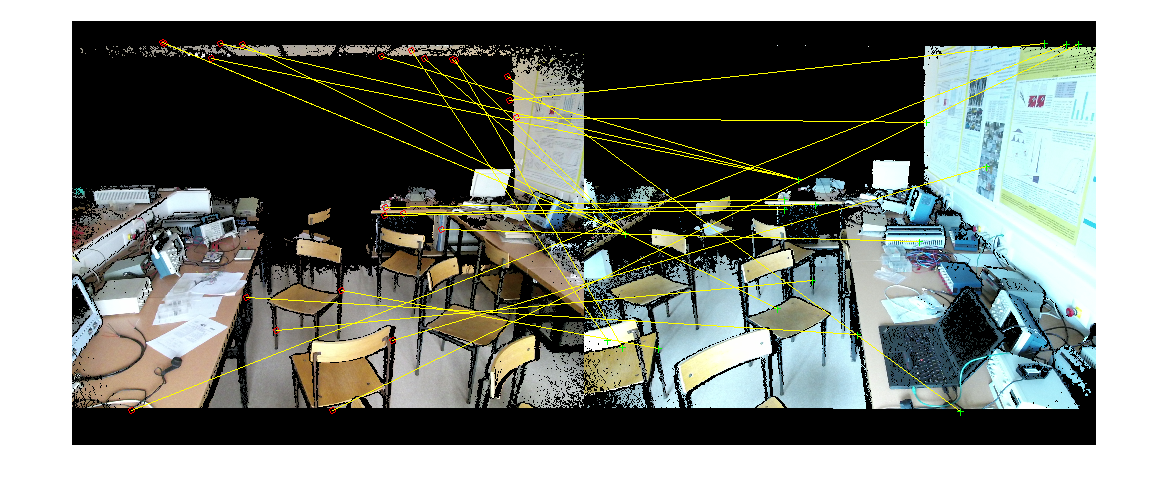
\includegraphics[width=\columnwidth]{./Slike/matched-features.png}
		\caption{Ujemajoče SURF značilke}
		\label{fig:zdruzevanje-surf}
	\end{subfigure}
	~
	\begin{subfigure}[t]{0.45\columnwidth}
		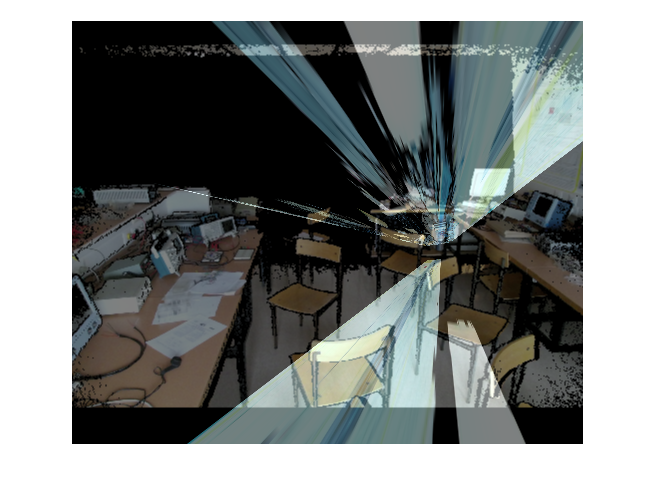
\includegraphics[width=\columnwidth]{./Slike/features-calibration-result.png}
		\caption{Rezultat združevanja z značilkami}
		\label{fig:zdruzevanje-result}
	\end{subfigure}
	\caption{Primer neuspelega poskusa združevanja slik iz dveh Kinect kamer s SURF značilkami.}
	\label{fig:zdruzevanje-znacilke}
\end{figure}

\paragraph{Združevanje s kontrolnimi točkami}
Zaporedja slik smo poskušali združiti z ročnim določevanjem kontrolnih točk. Rezultat je bil boljši od združevanja z značilkami, vendar še vedno slab, zato smo tudi to metodo opustili. Primer neuspelega poskusa je prikazan na sliki \ref{fig:zdruzevanje-cp}.

\begin{figure}[htb]
	\centering
	\begin{subfigure}[t]{0.45\columnwidth}
		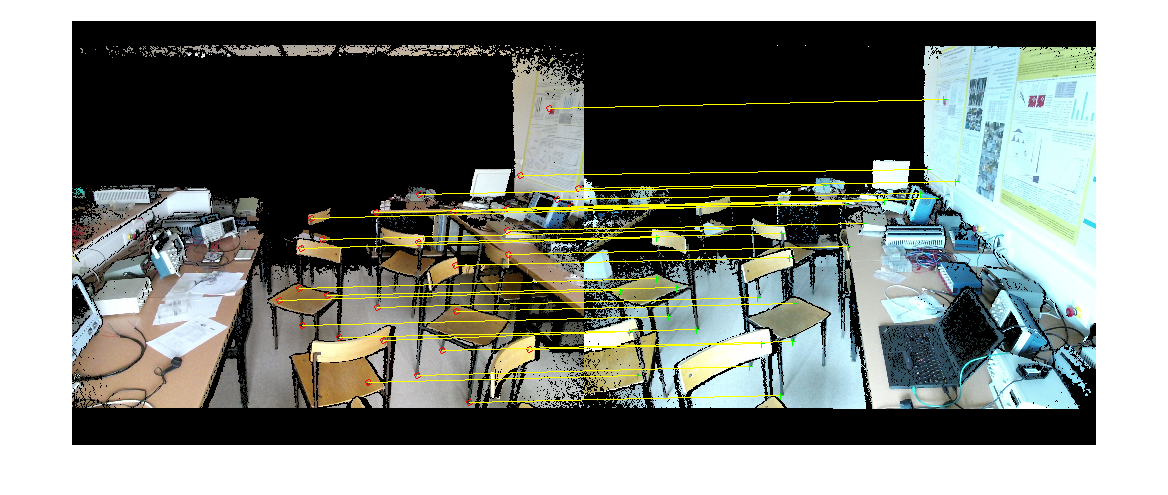
\includegraphics[width=\columnwidth]{./Slike/matched-points.png}
		\caption{Ujemajoče kontrolne točke}
		\label{fig:zdruzevanje-ujemajoce-cp}
	\end{subfigure}
	~
	\begin{subfigure}[t]{0.45\columnwidth}
		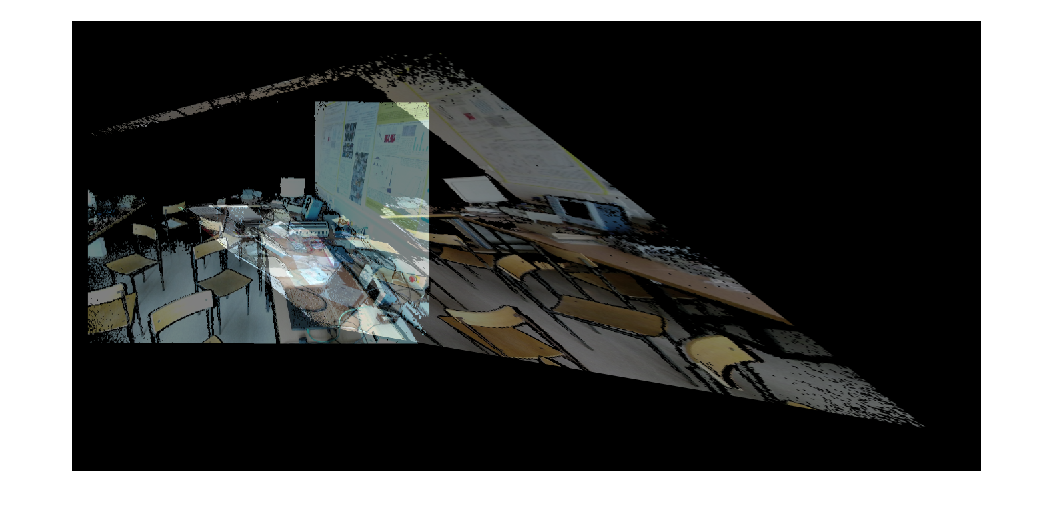
\includegraphics[width=\columnwidth]{./Slike/points-calibration-result.png}
		\caption{Rezultat združevanja s kontrolnimi točkami}
		\label{fig:zdruzevanje-result-cp}
	\end{subfigure}
	\caption{Primer neuspelega poskusa združevanja slik iz dveh Kinect kamer s kontolnimi točkami.}
	\label{fig:zdruzevanje-cp}
\end{figure}


\paragraph{Prilagojeno združevanje}
Zaradi nezadovoljivih rezultatov klasičnih metod združevanja stereo slik, smo razvili metodo, ki je prilagojena za Kinect kamere. Iz kamer smo pridobili intrinzične parametre infra-redečega (IR) senzora, in sicer: slikovni koordinati goriščne razdalje $f_u$ in $f_v$ ter slikovni koordinati optičnega središča slike (ang. principal point) $c_u$ in $c_v$. Intrinsične parametre smo uporabili za določitev intrizične matrike $\vec{M}_{int}$ po enačbi \eqref{eq:intrinsic}.


Ker pravih ekstrinsičnih parametrov kamer nismo poznali, smo jih le ocenili z metodo določevanja sečišča vidnih polj obeh kamer. Sečišče je prikazano kot rdeča linija na sliki \ref{fig:zdruzevanje}. S to metodo smo določili translacijski vektor $\vec{t} = \left [ t_x~ t_y~ t_z \right]^\top$ in rotacijsko matriko $\vec{R}$ iz Eulerjevih kotov.

S sledenjem igralca z DS-KCF algoritmom, smo s pomočjo projekcijske matrike \eqref{eq:projection-matrix} določili center tarče v metričnih enotah za vsako sliko zaporedja leve in desne kamere. Kadar slikovni element ni vseboval podatkov globine, smo za center tarče izbrali najbližji slikovni element z veljavno globino.

Prva slika združenega zaporedja je bila slika kamere, kjer se igralec prvič pojavi. Nadaljne slike smo izbirali med zaporedjema kamer glede na pozicijo centra tarče. Ko je šel center tarče skozi upragovljeno mejo, ki je na sliki \ref{fig:zdruzevanje} prikazana z modro linijo smo preklopili na drugo kamero. Razdalja med pragom in sečiščem je znašala \SI{200}{mm}.


\begin{figure}[htb]
	\centering
	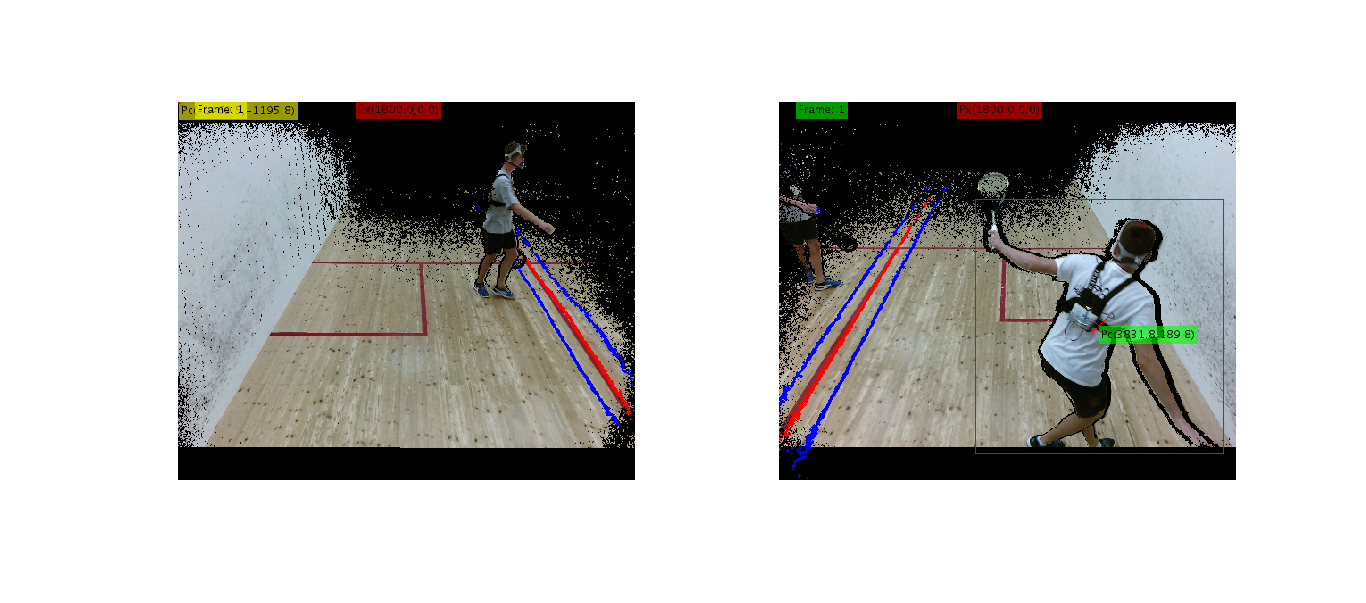
\includegraphics[width=\columnwidth]{./Slike/zdruzevanje-example.png}
	\caption[Določevanje sečišča vidnih polj leve in desne Kinect kamere]{Določevanje sečišča vidnih polj leve in desne Kinect kamere. Na sliki sta prikazani prvi sliki zaporedja leve in desne Kinect kamere 1. seta 2. igre terenskega eksperimenta iz 2. faze. Označen je 4. igralec. Zelena barva koordiat središča tarče predstavlja izbrano kamero. Kamera z rumeno barvo ni izbrana. Sečišče je rdeča linija. Modri liniji sta pragova za preklop med kamerama. Ležita \SI{200}{mm} levo in desno od sečišča.}
	\label{fig:zdruzevanje}
\end{figure}





\subsubsection{Regresija \texorpdfstring{$\nu$}{nu}-RBF}
dodali 



\subsubsection{Optimizacija Gaussovega filtra}
Pri optimizaciji Gaussovega filtra smo določili optimalni standardni odklon $\sigma$ z uporabo dveh metrik, in sicer: koren srednje kvadratične napake (RMSE) in razmerje med signalom in šumom (SNR). Pri RMSE metriki smo določili napako med učnimi vzorci in njihovo predikcijo. Pri SNR metriki smo za signal uporabili referenčne učne vzorce. Za šum smo uporabili rezidualni ali preostali šum. Tega smo dobili z odštevanjem filtriranih vzorcev od referenčnih. SNR metrika tako določa uspešnost izločevanja šuma, RMSE metrika pa pravilnost določevanja kateri podatki spadajo v signal in kateri v šum.


Teste smo izvajali na vseh eksperimentih 1. sklopa, pri čemer smo uporabili $\nu$-RBF jedro s \SI{50}{\%} podpornih vektorjev. Za filtriranje pri mrežnem iskanju smo izbrali najmanjši filter s $\sigma = 1$. Testirali smo naslednje standardne odklone Gaussovega filtra: $1, 3, 5, 11, 21, 31$ in $51$. 

Rezultati povrprečnih vrednosti uporabljenih metrik so vidni v tabeli \ref{tab:gauss}. Za pravilno razlago rezultatov, moramo upoštevati tudi grafe metrik posameznih eksperimentov, ki so prikazani na slikah \ref{fig:sigma1-5}, \ref{fig:sigma-rmse5-21} in \ref{fig:sigma21-51}. 



\begin{table}[htb]
	\centering
    \begin{tabular}{S[table-format=2.0] S[table-format=2.3] S[table-format=2.3]}
    \toprule
    \thead{$\mathbf{\sigma}$} & \thead{RMSE} & \thead{SNR [dB]}  \\
    \midrule%nSV
    1 & \boldentry{2.3}{8.614} & 24.278 \\
    3 & 11.236 & 25.470 \\
    \boldentry{2.0}{5} & 11.596 & 25.746 \\
    11 & 11.783 & 25.746 \\
    21 & 11.842 & 25.975 \\
    31 & 11.871 & 26.194 \\
    51 & 11.907 & \boldentry{2.3}{26.306} \\
    \bottomrule
    \end{tabular}
    \caption[Povprečne vrednosti RMSE in SNR metrik pri optimizaciji parametra $\sigma$ Gaussovega filtra]{Povprečne vrednosti RMSE in SNR metrik pri optimizaciji parametra $\sigma$ Gaussovega filtra. Najmanjši standardni odklon ima najmanjšo napako, vendar je tudi filtriranje majhno. Pri $\sigma=3$ in $\sigma=5$ so še opazne razlike pri filriranju. Za višje vrednosti ni več opazne razlike, vendar pa se napaka povečuje. $\sigma=5$ je tako optimalna vrednosti parametra.}
    \label{tab:gauss}
\end{table}

Najmanjšo napako dobimo, če uporabimo $\sigma=1$, vendar pa imamo pri tem najmanjše filtriranje, zato so rezultati še vedno lahko zelo šumni. Z višanjem parametra filtra, se napaka po metriki RMSE povečuje, vendar ima večji vpliv razmerje SNR, saj je predstavljeno v logaritemski skali. 

\begin{figure}[!htb]
\centering
\begin{subfigure}[t]{0.45\columnwidth}
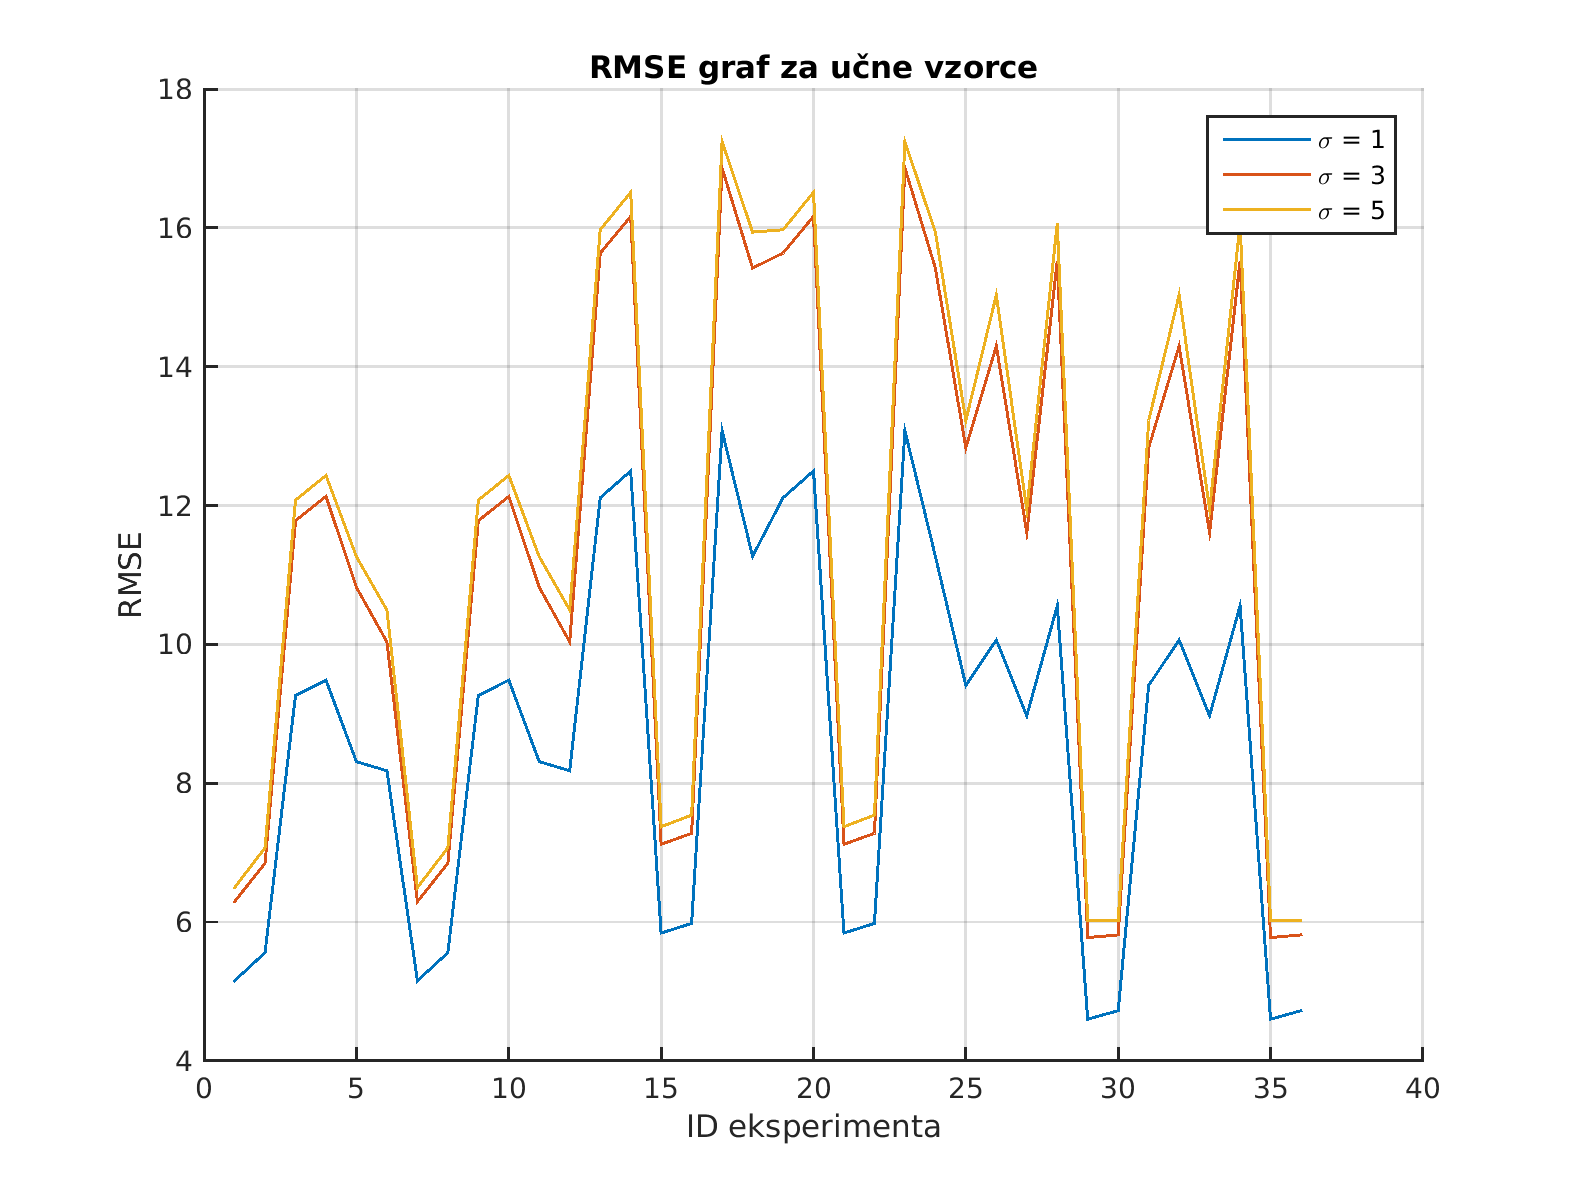
\includegraphics[width=\columnwidth]{./Slike/sigma-rmse1-5.png}
\caption{Graf RMSE  učnih vzorcev }
\label{fig:sigma-rmse1-5}
\end{subfigure}
~
\begin{subfigure}[t]{0.45\columnwidth}
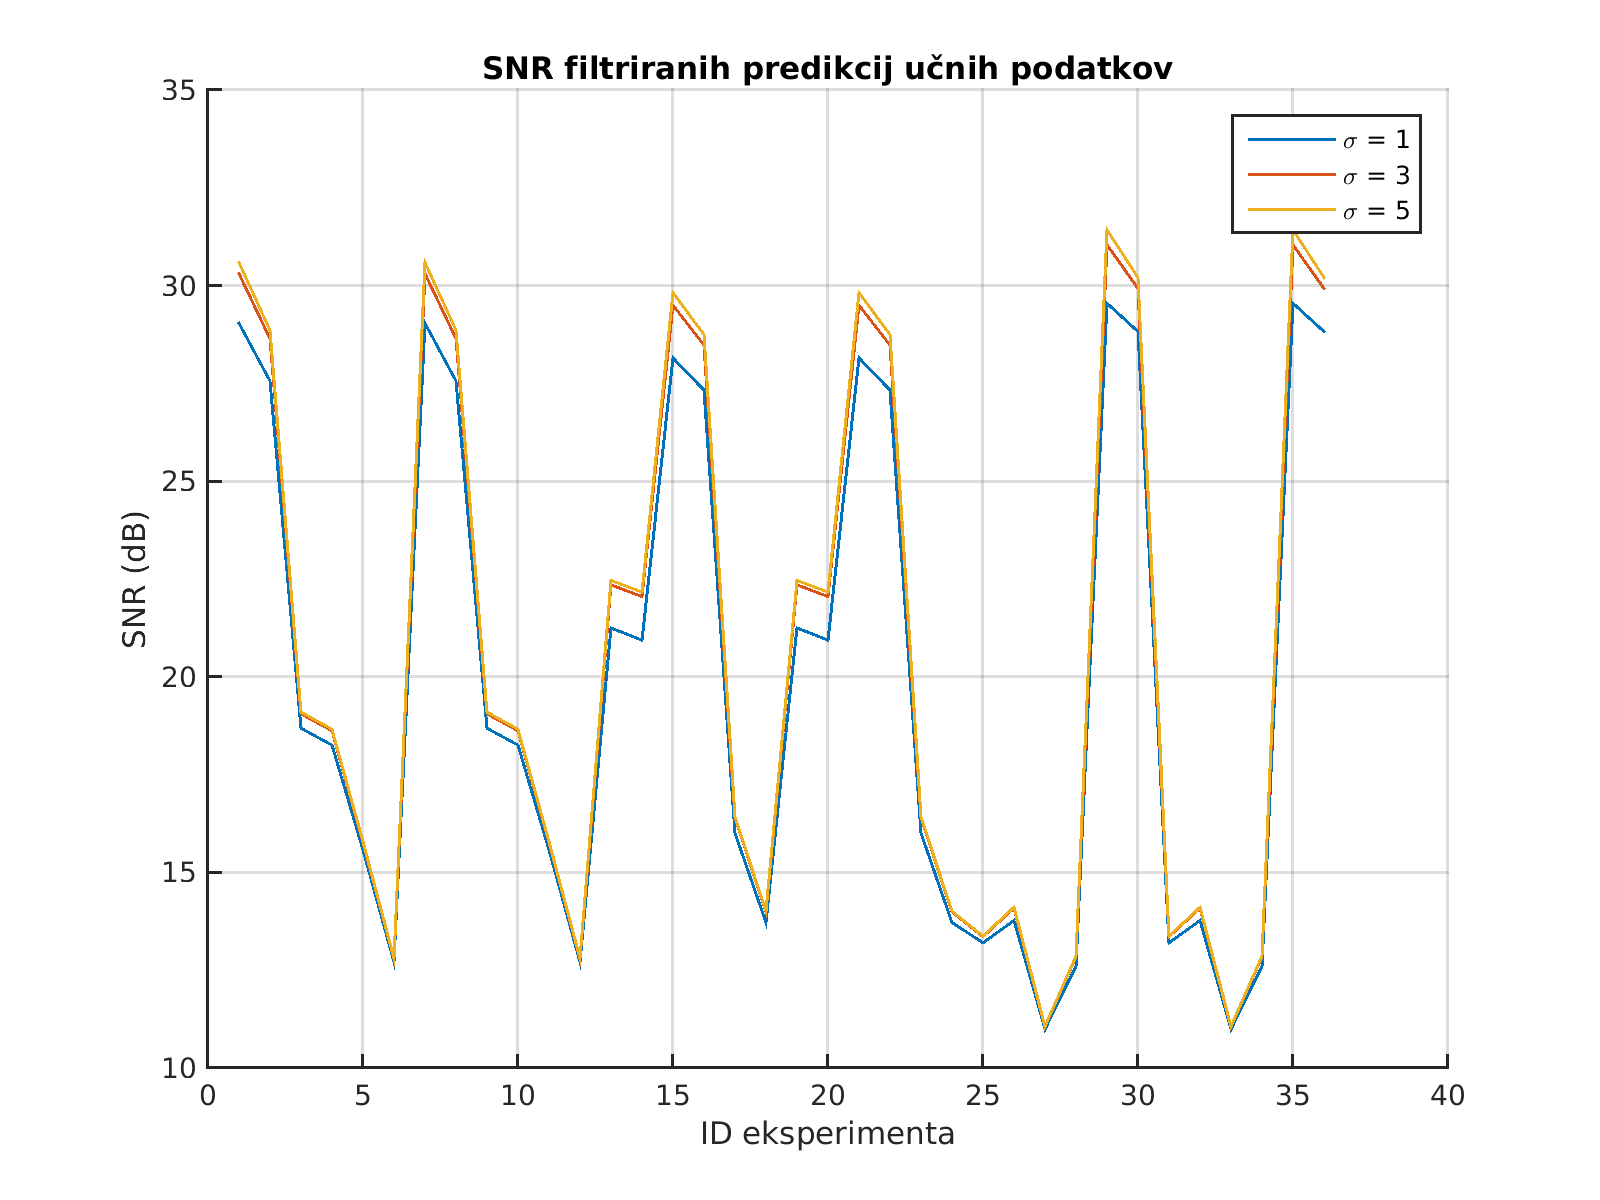
\includegraphics[width=\columnwidth]{./Slike/sigma-snr1-5.png}
\caption{Graf SNR  učnih vzorcev}
\label{fig:sigma-snr1-5}
\end{subfigure}
\caption{Grafa RMSE in SNR učnih vzorcev za \mbox{$\sigma \in [1,5]$}}
\label{fig:sigma1-5}
\end{figure}

Čeprav pri uporabi $\sigma=51$ dobimo največje filtriranje šuma, lahko na slikah grafov opazimo, da se obe metriki bistveno ne razlikujeta za vrednosti parametra na intervalu $[5,51]$. Kljub dobremu filtriranju želimo zagotoviti čim manjšo napako med referenčnim signalom in predikcijo, zato je logična izbira čim manjši standardni odklon. Ker so na sliki \ref{fig:sigma1-5} med $\sigma=3$ in $\sigma=5$ še opazne razlike, lahko zaključimo, da je $\sigma=5$ optimalna izbira parametra za naš problem. 


\begin{figure}[htb]
\centering
\begin{subfigure}[t]{0.45\columnwidth}
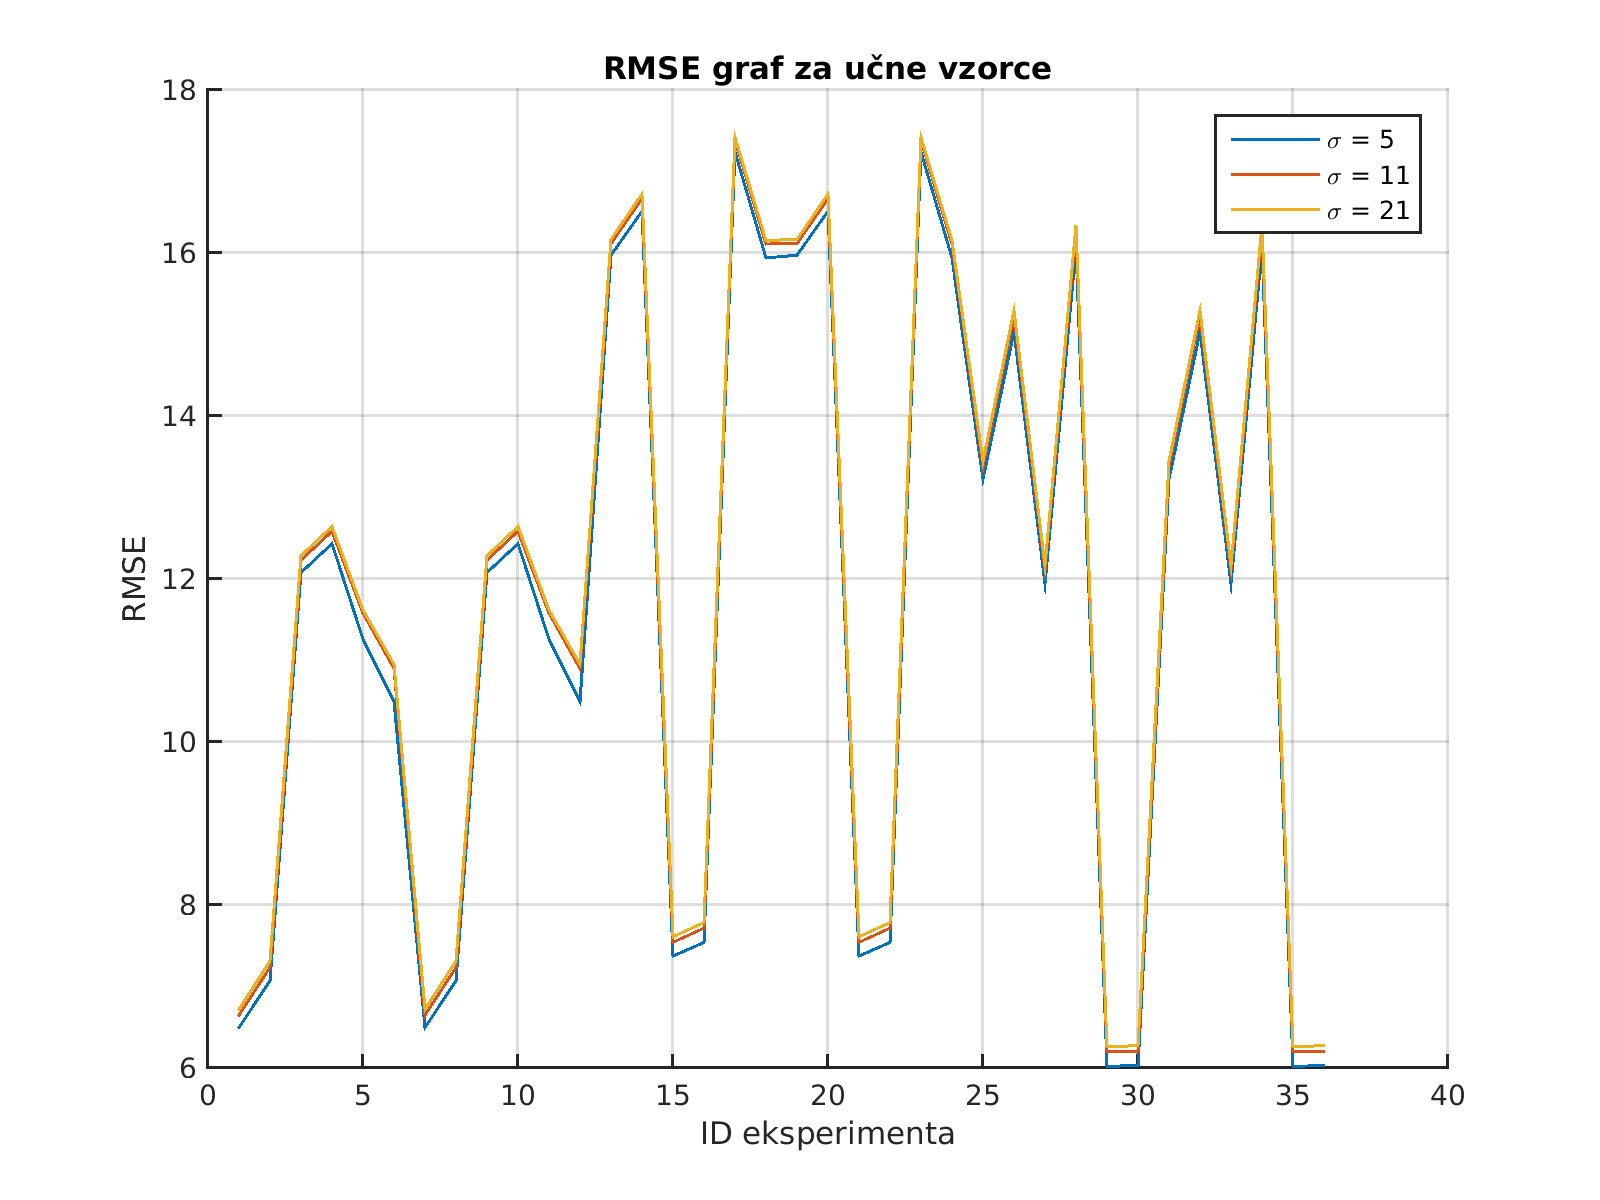
\includegraphics[width=\columnwidth]{./Slike/sigma-rmse5-21.png}
\caption{Graf RMSE  učnih vzorcev}
\label{fig:sigma-rmse5-21}
\end{subfigure}
~
\begin{subfigure}[t]{0.45\columnwidth}
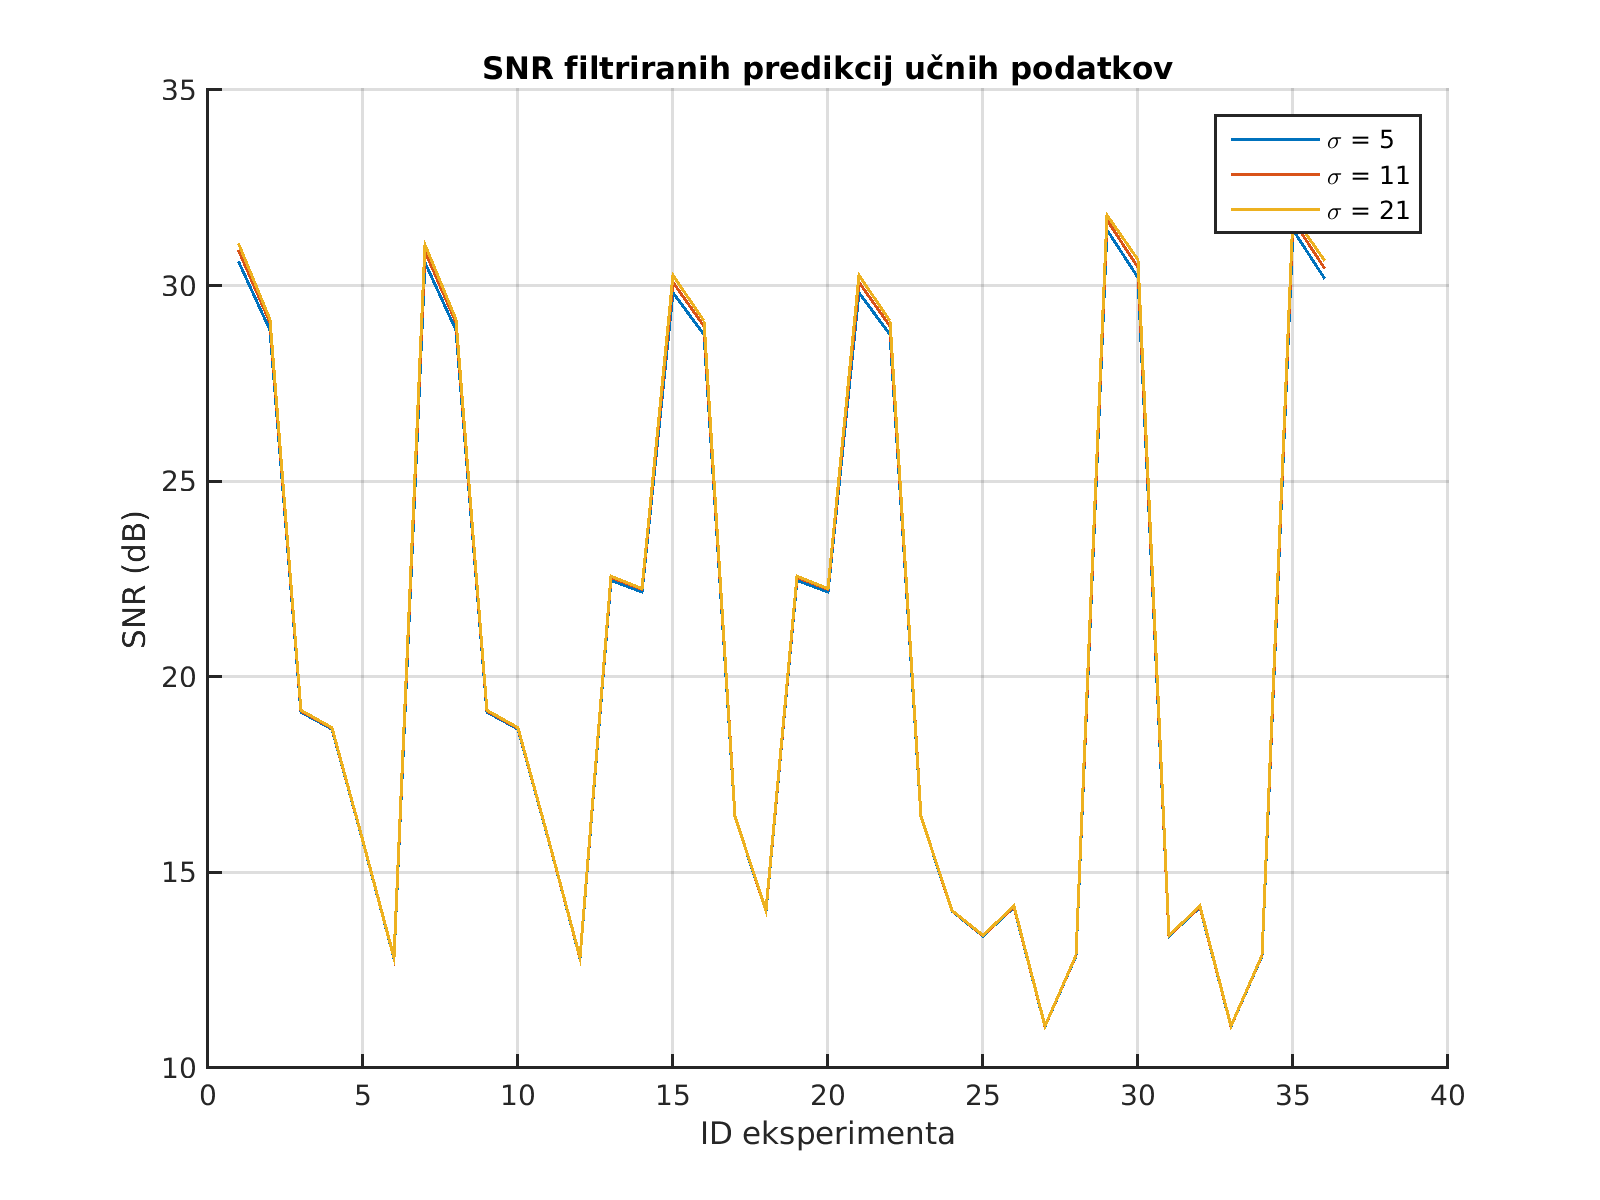
\includegraphics[width=\columnwidth]{./Slike/sigma-snr5-21.png}
\caption{Graf SNR  učnih vzorcev}
\label{fig:sigma-snr5-21}
\end{subfigure}
\caption{Grafa RMSE in SNR učnih vzorcev za \mbox{$\sigma \in [5,21]$}}
\label{fig:sigma5-21}
\end{figure}



\begin{figure}[htb]
\centering
\begin{subfigure}[t]{0.45\columnwidth}
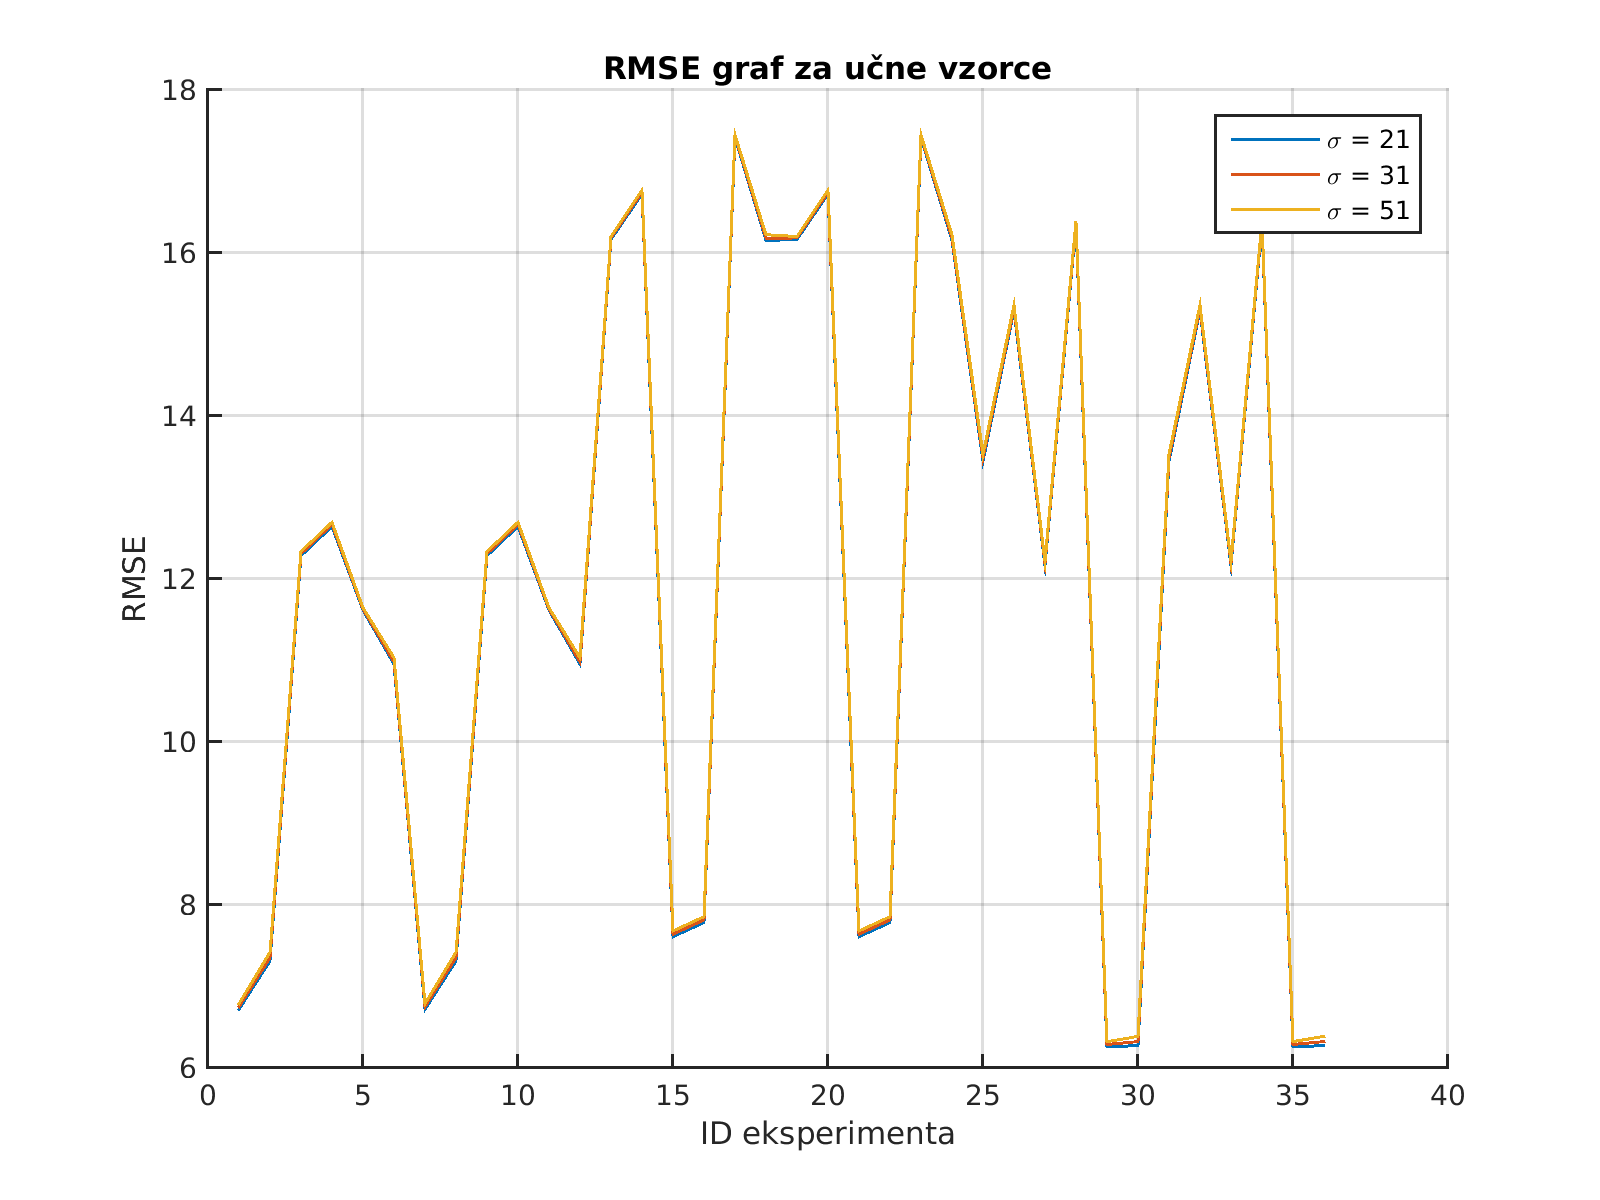
\includegraphics[width=\columnwidth]{./Slike/sigma-rmse21-51.png}
\caption{Graf RMSE učnih vzorcev}
\label{fig:sigma-rmse21-51}
\end{subfigure}
~
\begin{subfigure}[t]{0.45\columnwidth}
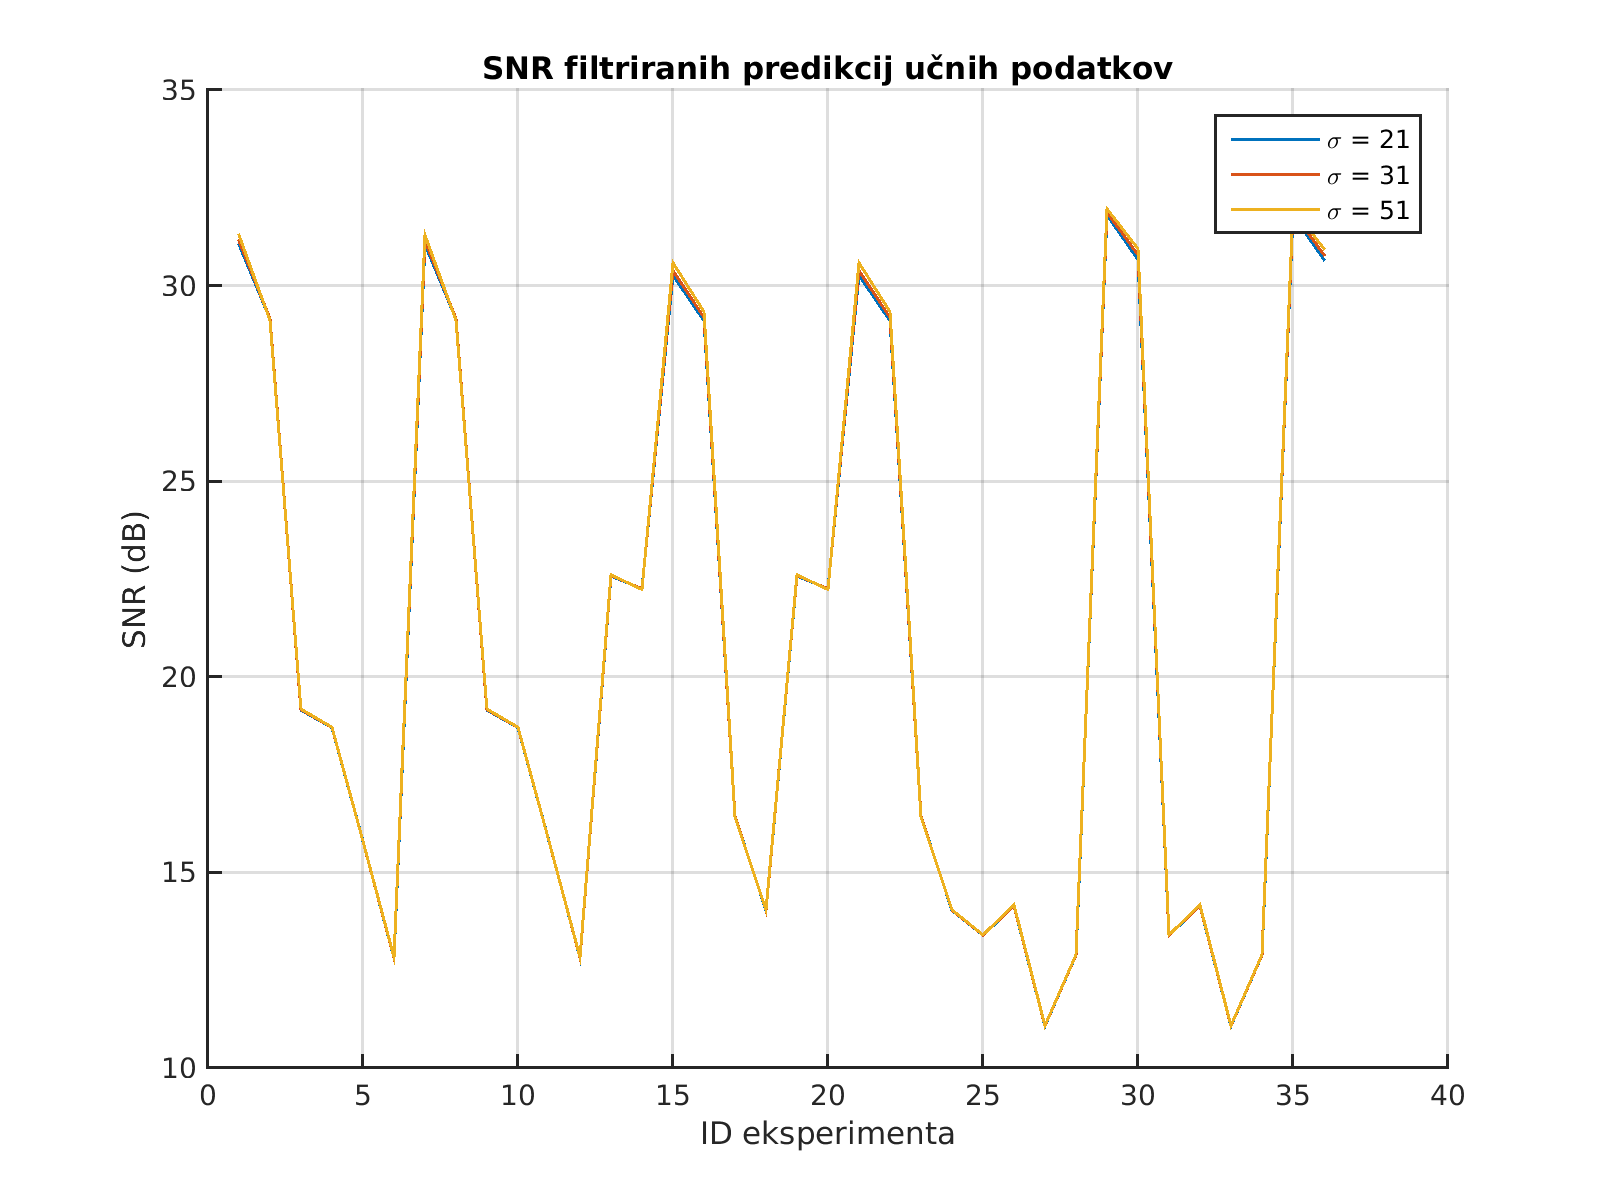
\includegraphics[width=\columnwidth]{./Slike/sigma-snr21-51.png}
\caption{Graf SNR  učnih vzorcev}
\label{fig:sigma-snr21-51}
\end{subfigure}
\caption{Grafa RMSE in SNR učnih vzorcev za \mbox{$\sigma \in [21,51]$}}
\label{fig:sigma21-51}
\end{figure}



\subsubsection{Normalizacija HAFA deskriptorjev}
% Zakaj naj bi bila ta rešitev dobra
% teorija tovrstne kalibracije
% Kako s to kalibracijo nismo popravili stvari
% In da smo ugotovili da obstaja še prostorski tok, ki bi nam rešil težave
!!!!!!!!!!!!!!!!!!!!!!!!!!!!!!!

V praksi se pokaže, da normiran HAFA histogram ne... -> To paše pod eksperimente.

!!!!!!!!!!!!!!!!!!!!!!!!!!!!!!!!!!!!!!!!!


\subsection{Laboratorijski eksperimenti}
"Opis testa Nowatzky "

Merjenci  so opravili obremenilni test po protokolu Nowatzky. To je stopnjevani test na tekoči preprogi za merjenje maksimalne porabe kisika in oceno aerobne kapacitete  posameznika. Test smo izvajali s pomočjo sistema za direktno ergospirometrijo tipa ``breath  by breath'' Cosmed K4B2. Uporabili smo  tekočo  preprogo HP Cosmos. Test smo pričeli z ogrevanjem 3 minute s hitrostjo teka 5 km/h, pri naklon preproge 0 \%. Nadaljevali smo s 3 minutnim tekom s hitrostjo 6 km/h. Po treh minutah smo naklon tekoče preproge  dvignili za 2 \% in ga nismo več spreminjali. Po pretečeni minuti na  tretji stopnji (hitrost 6; naklon 2 \%) se je hitrost teka vsaki dve  minuti  povečevala za 1 km/h. Test smo izvajali brez prekinitve do pojava objektivnih oz. subjektivnih razlogov za prekinitev testa. Po koncu testiranja je sledilo še 5 min hoje pri  hitrosti 2 km/h ter 0 \% naklonu.  

\subsubsection{Določitev zakasnitve fiziološkega odziva}
\begin{figure}[!htbp]
	\centering
	\begin{subfigure}[t]{0.45\columnwidth}
		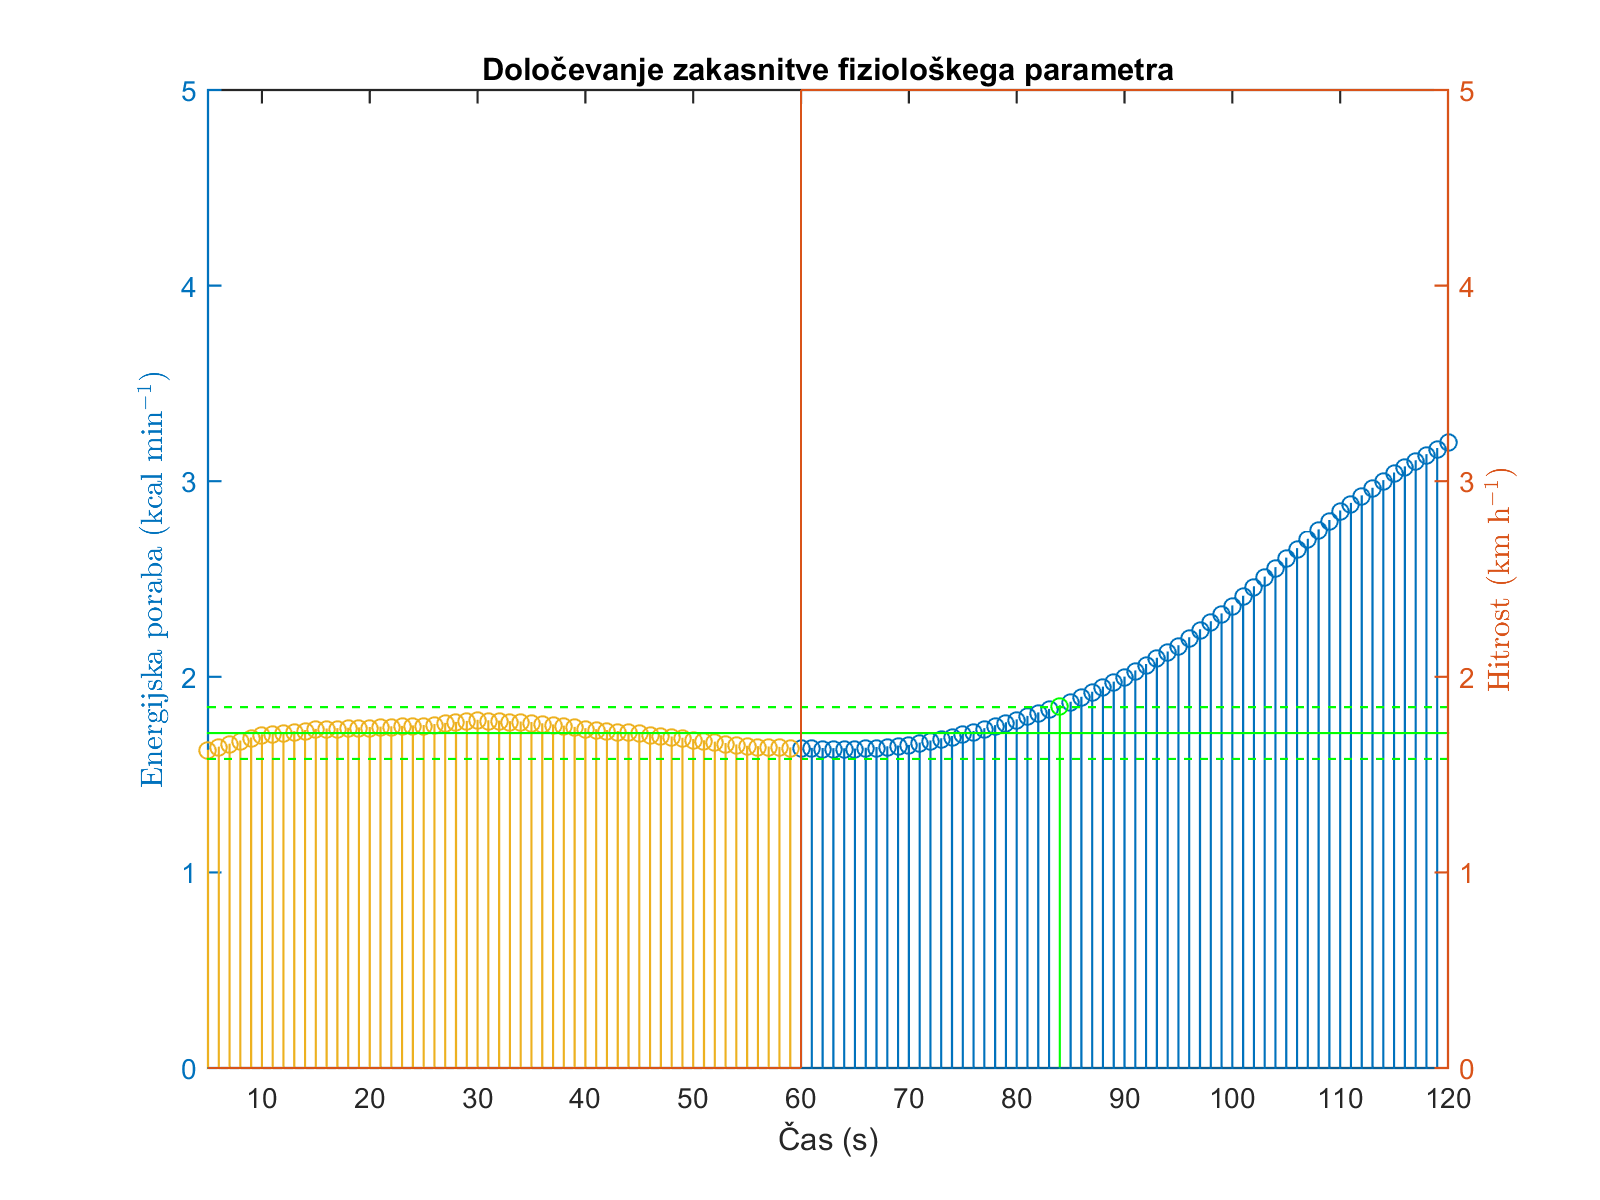
\includegraphics[width=\columnwidth]{./Slike/lag-estimation-1-eem.png}
		\caption{Zakasnitev za subjekt 1.}
		\label{fig:lag-estimation-1-eem}
	\end{subfigure}
	~
	\begin{subfigure}[t]{0.45\columnwidth}
		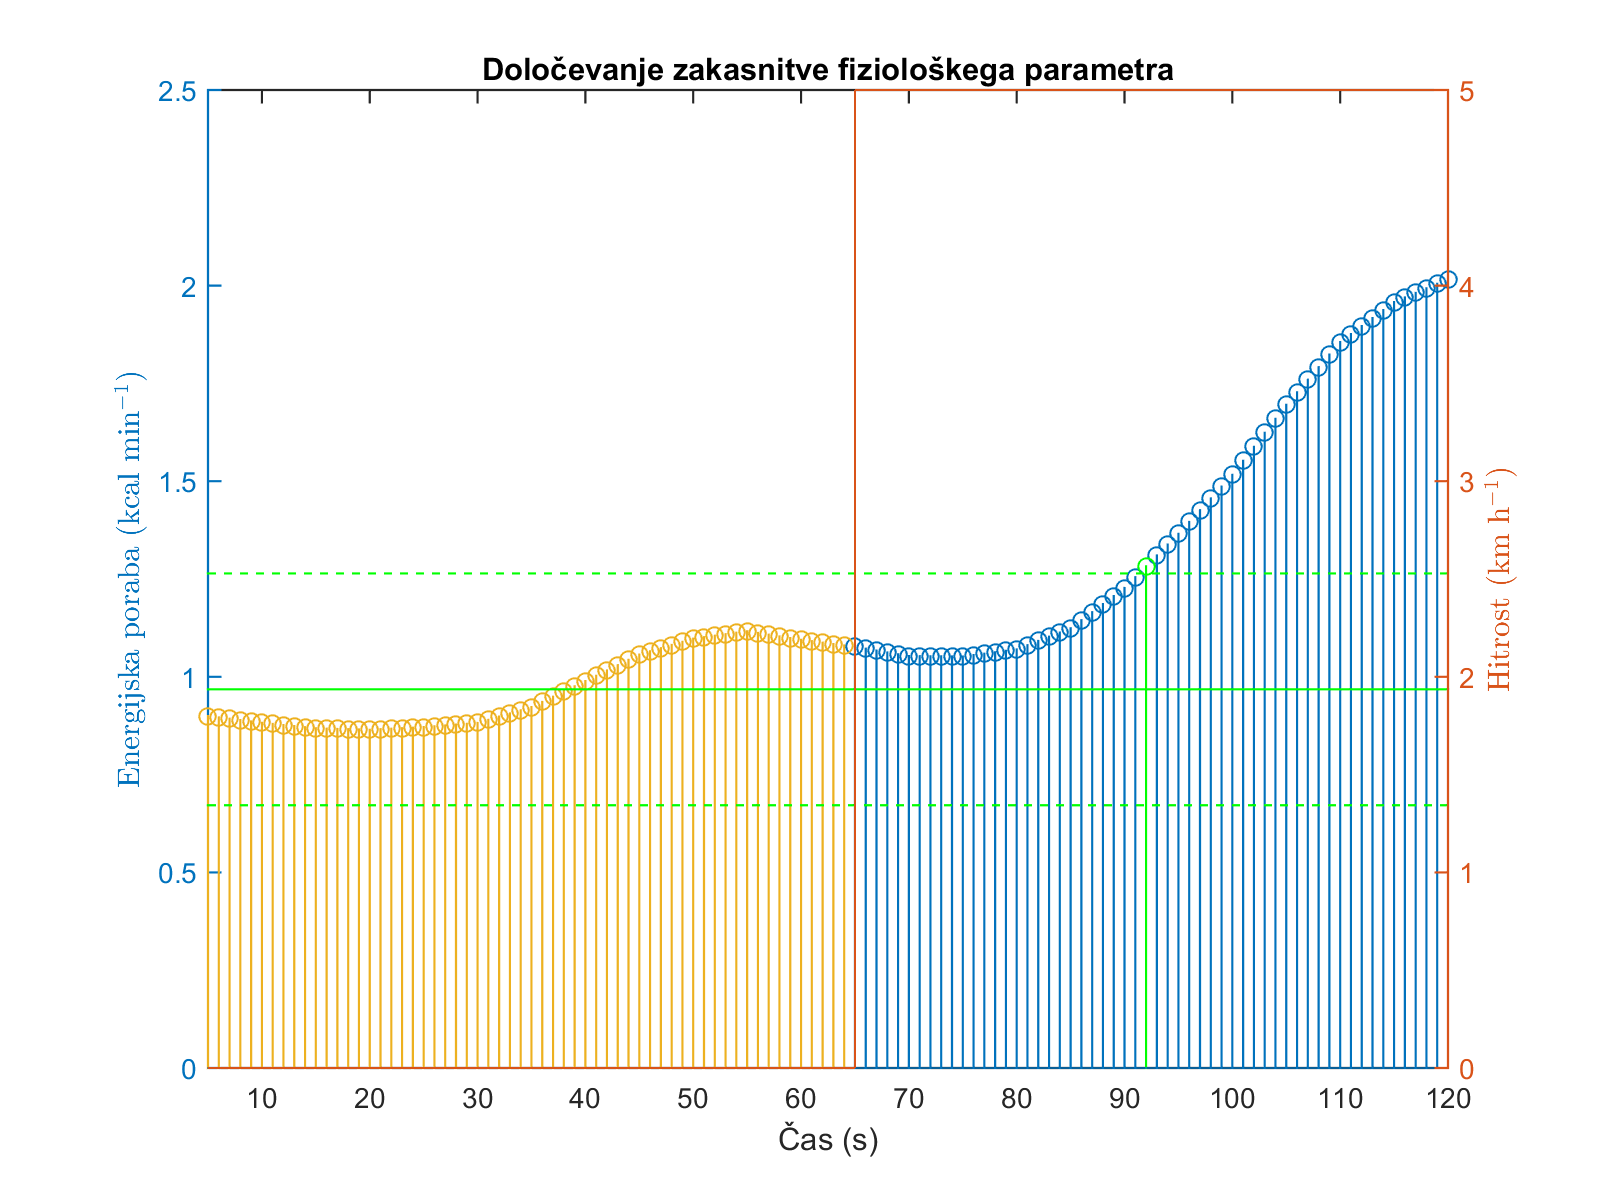
\includegraphics[width=\columnwidth]{./Slike/lag-estimation-2-eem.png}
		\caption{Zakasnitev za subjekt 2.}
		\label{fig:lag-estimation-2-eem}
	\end{subfigure}
	~
	\begin{subfigure}[t]{0.45\columnwidth}
		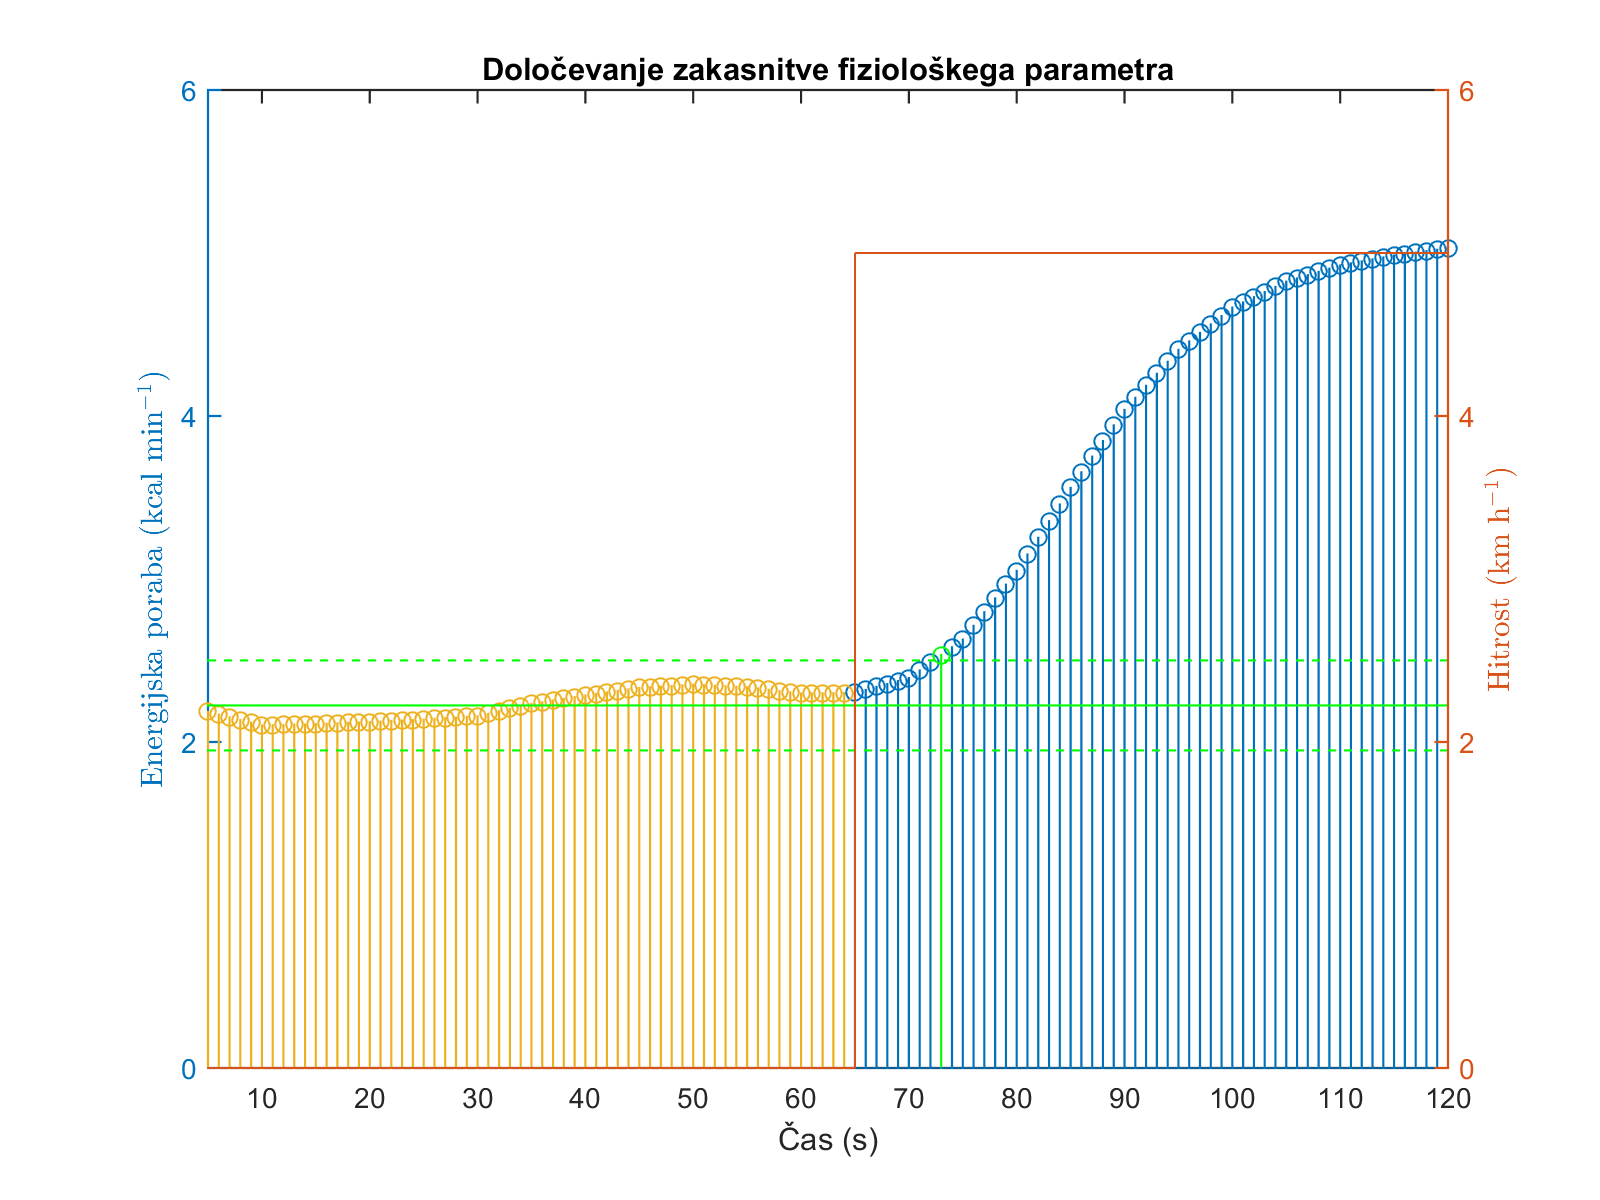
\includegraphics[width=\columnwidth]{./Slike/lag-estimation-3-eem.png}
		\caption{Zakasnitev za subjekt 3.}
		\label{fig:lag-estimation-3-eem}
	\end{subfigure}
	~
	\begin{subfigure}[t]{0.45\columnwidth}
		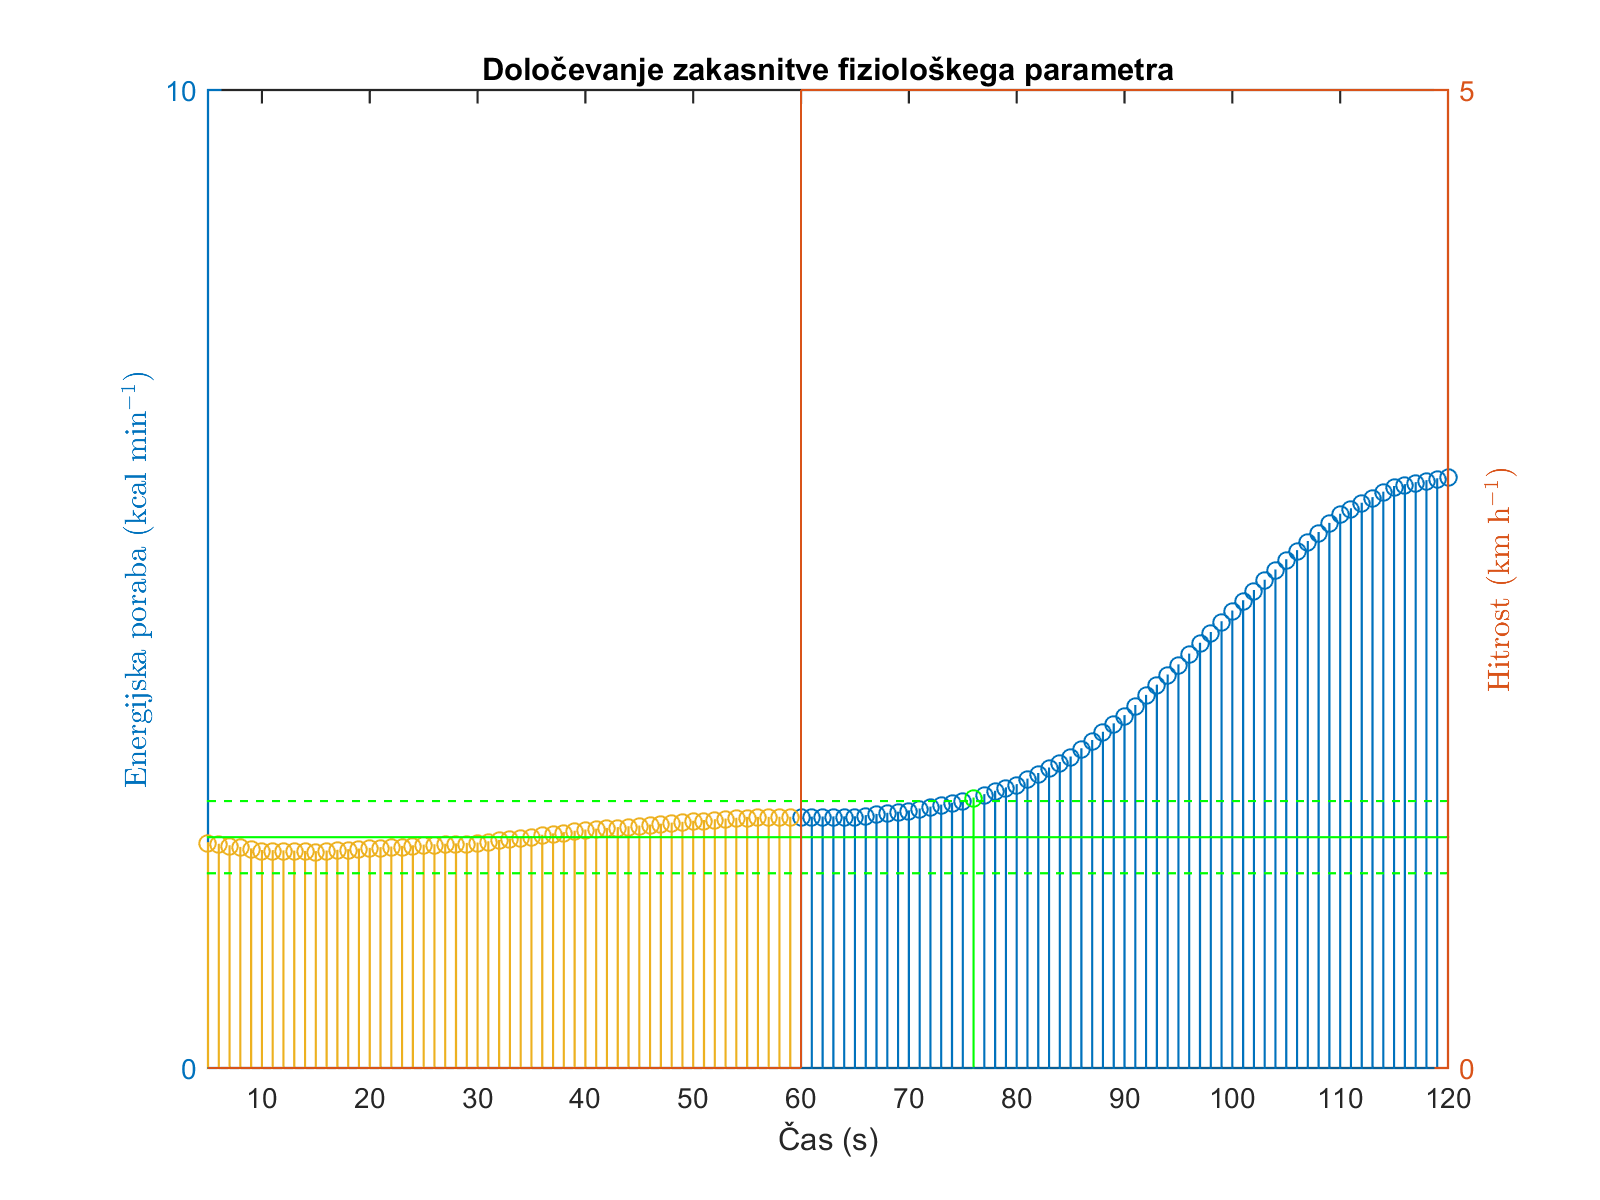
\includegraphics[width=\columnwidth]{./Slike/lag-estimation-4-eem.png}
		\caption{Zakasnitev za subjekt 4.}
		\label{fig:lag-estimation-4-eem}
	\end{subfigure}
	~
	\begin{subfigure}[t]{0.45\columnwidth}
		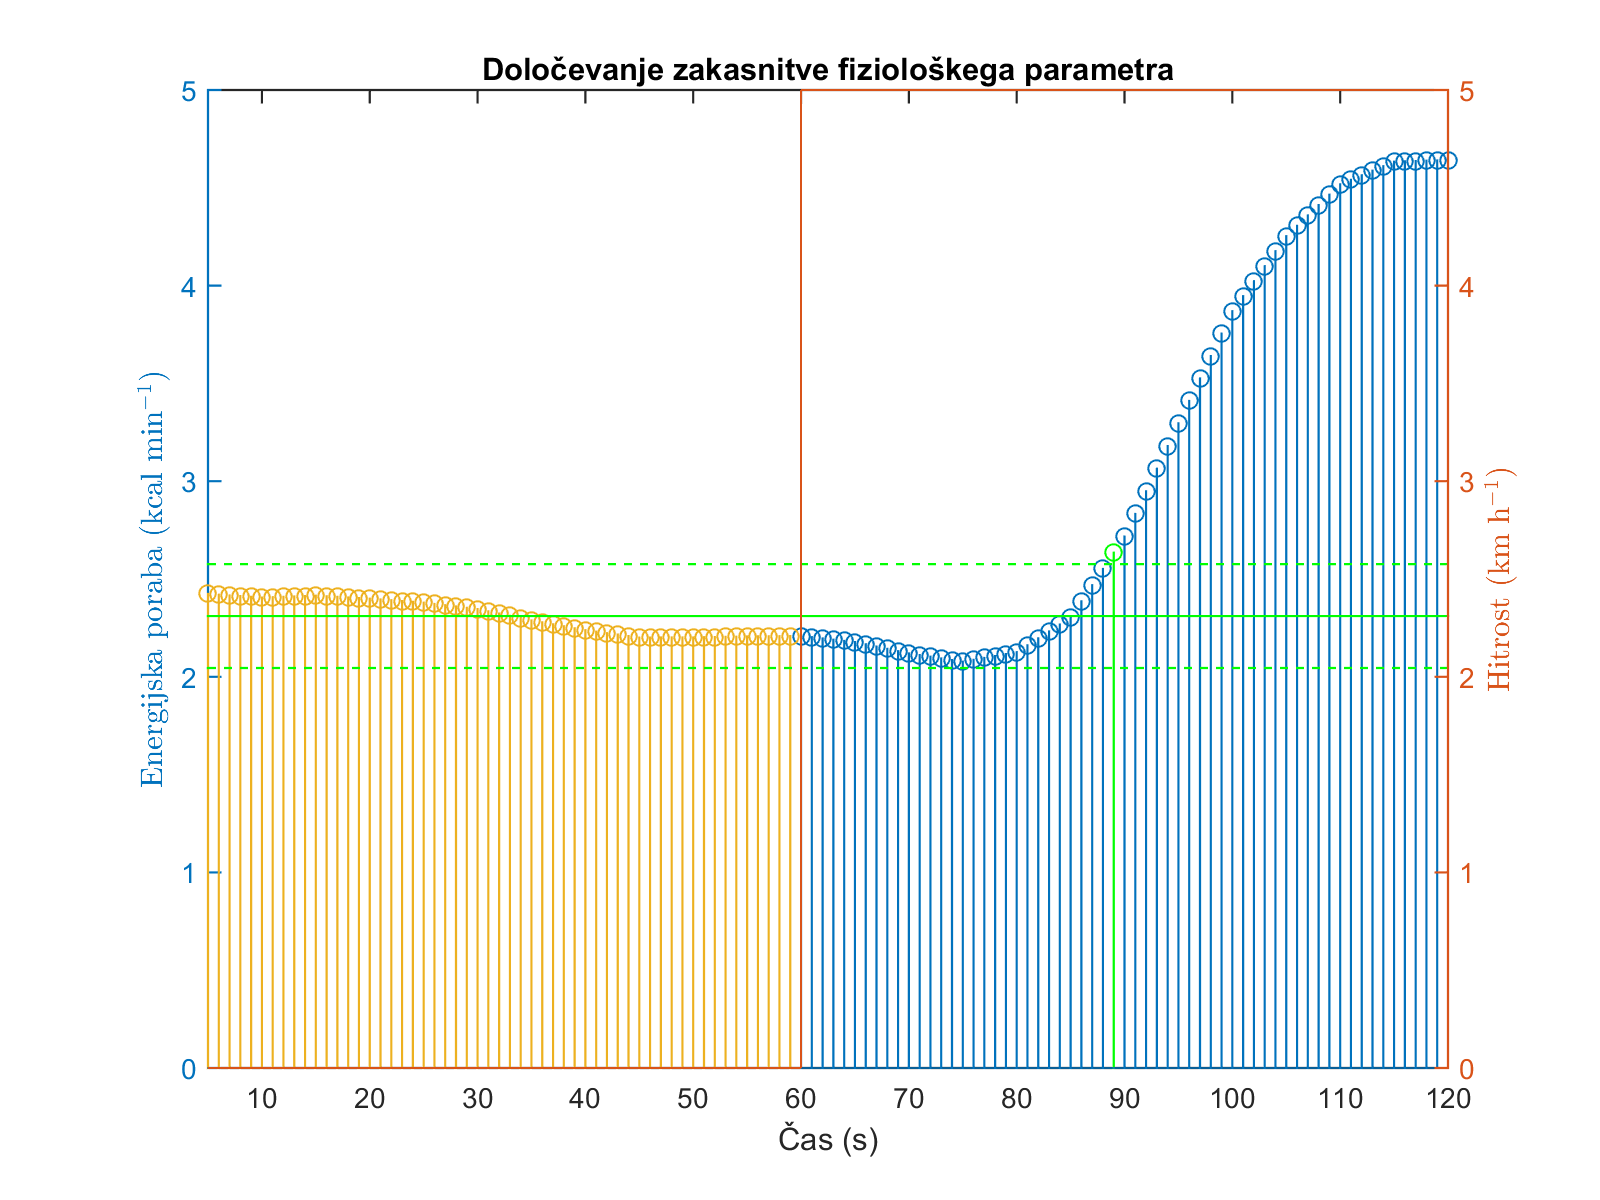
\includegraphics[width=\columnwidth]{./Slike/lag-estimation-5-eem.png}
		\caption{Zakasnitev za subjekt 5.}
		\label{fig:lag-estimation-5-eem}
	\end{subfigure}
	~
	\begin{subfigure}[t]{0.45\columnwidth}
		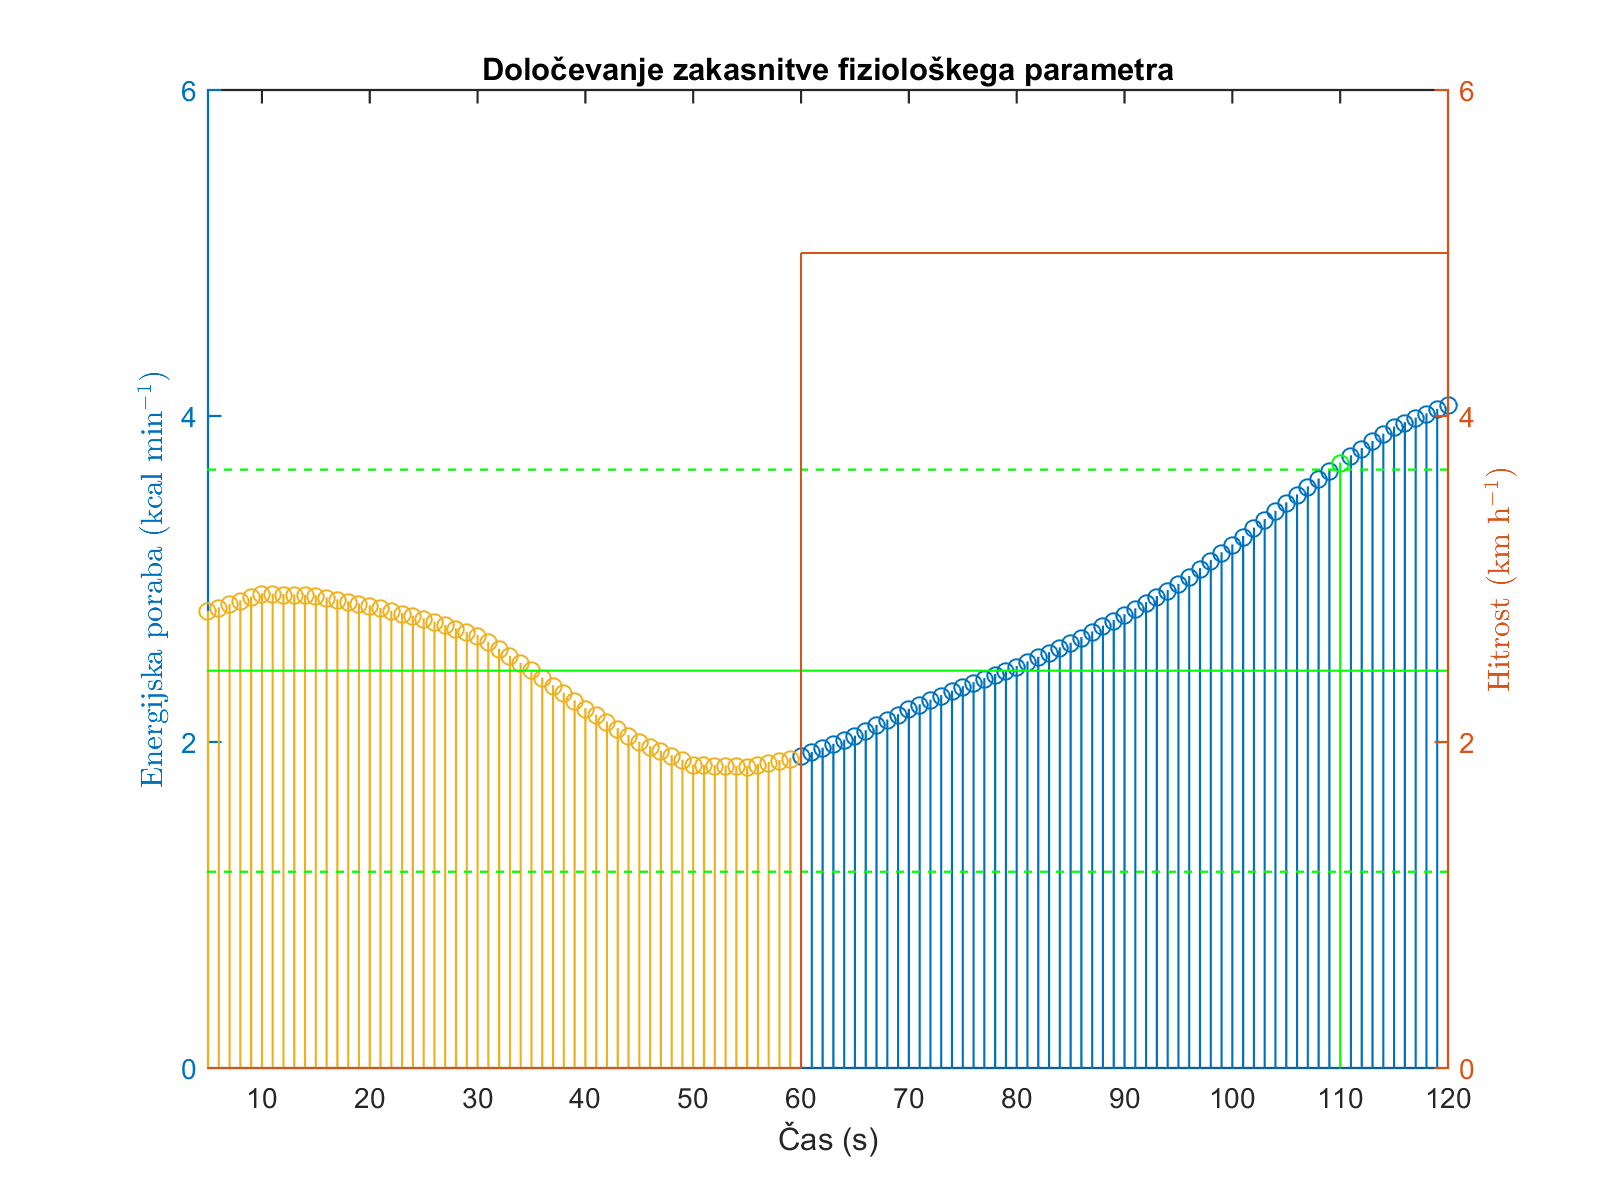
\includegraphics[width=\columnwidth]{./Slike/lag-estimation-6-eem.png}
		\caption{Zakasnitev za subjekt 6.}
		\label{fig:lag-estimation-6-eem}
	\end{subfigure}
	\caption{}
	\label{fig:lag-estimation-stage2}
\end{figure}

\subsection{Terenski eksperimenti}
a
